%%
%%
%% This file should be edited by user
%%

\chapter{tinyos} \label{chapter:tinyos}

\section{tinyOS Basics}

\subsection{What is tinyOS}

tinyOS is a free and open operating system for hardware motes, which is written in nesC. A hardware mote is a microcontroller based node in a wireless sensor network, capable of reading sensory information, processing and exchanging of this data with other nodes. Communication typically goes on over wireless network, because so the cost for deployment and maintenance is reduced, and because wires are not feasible in many environments. 

Development of tinyOS started as a collaboration of Berkeley University with Intel Research and Crossbow Technology, a california based company.
The following requirements were defined for tinyOS:

\begin{itemize}
 \item Require very few resources
 \item Allow fine-grained concurrency
 \item Adapt to hardware evolution
 \item Support a wide range of applications
 \item Robust Design
 \item Support a diverse set of platforms
\end{itemize}

One of tinyOS's most important features is that tinyOS applications are built out of components, which are connected or wired to each other by interfaces. Components can easily be developed, extended and reused. Another advantage is that a component can be built in software \textbf{or} hardware, increasing flexibility. But because hardware is always non-blocking, the software must be non-blocking as well to guarantee this exchangeability. So, tinyOS uses the split-phase - model: a userprogram that wants to execute some kind of code \textit{posts} a \textit{task}, which is queued by the task scheduler, and gets executed later. The finished execution of the task is afterwards \textit{signaled} to the caller of the task. This behavior can be compared to a hardware interrupt: some kind of operation is requested by a program, so the program initialises the needed datastructures and starts the operation. But instead of waiting until the hardware has finished, the userprogram returns immediatly and continues with other instructions, and gets discontinued by an interrupt as soon as the hardware has finished.

\section{History}

Developement of tinyOS started in 1999 at Berkeley university. The first supported platform was a mote 
called 'WeC', as shown in figure~\ref{fig:WeC}. For communication, this platform is equipped wit an radio device and SPI and UART - interfaces. As cpu an Atmel AVR AT90LS8535 microprocessor, clocked with 4MHz, is used. A major advantage of this mote is that it can be programmed over the wireless interface.
\begin{figure}[h]
 \centerline{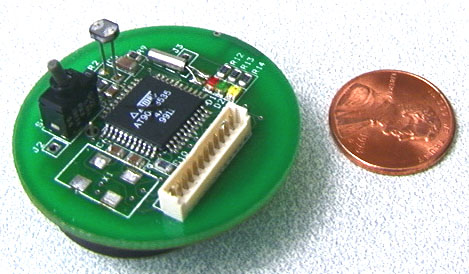
\includegraphics[width=.5\columnwidth]{pics/WeC.png}}
  \caption{WeC Mote}
  \label{fig:WeC}
\end{figure}

In the next years, the 'rene' and 'mica' platforms are developed. In the year 2002, work on the nesC programming language began. Until that, tinyOS consisted of a mixture of C files and Perl scripts. In the same year, tinsOS 1.0, the first tinyOS implemented in nesC, is released. 

Improvement of tinyOS 1.x went on until february 2006, when tinyOS 2.0 beta1 was released. Version 2.1 was finished in april 2007. Among numerous bugfixes, a cc2420 wireless radio stack implementation was added in this release. tinyOS 2.02 was released some months later, which included an cc2420 stack reimplementation and bugfixes.
After that, in august 2008, support for the 'iris' and 'shimmer' platforms was added by distribution of version 2.1. Clearly, bugfixes were included in this release too.

At the time of this writing, the latest tinyOS version is 2.1.1, which was released in April 2010. Most important add-ons are support for the 'mulle', 'epic' and 'shimmer2' - platforms. 

\section{Supported Platforms}

With version 2.1.1, a range of hardware motes are supported out-of-the-box. A brief description of this platforms and its most important communication devices are given in the following list. Obviously, most of this platforms provide interfaces for UART, I2C, SPI or others peripherals, depending of the microcontroller and extension boards used, too. These features are not listed here.

\begin{itemize}
 \item btnode3: Atmega128L cpu and radio/bluetooth communication devices
 \item epic: MSP430 cpu and CC2420 radio chip
 \item eyesIFX: MSP430F149/F1611 and TDA5250 wireless transceiver
 \item intelmote2: PXA271 XScale cpu and CC2420 radio chip 
 \item mica: Atmega103 and TR1000 radio chip
 \item mica2: Atmeage128L and Chipcon 868/916 radio chip
 \item mica2dot: Atmega128 and cc1000 transceiver
 \item micaz: Atmega128 and cc2420 radio chip
 \item mulle: Renesas M16C and AT86RF230 transceiver
 \item sam3s\_ek: SAM3S4C chip and cc2520 transceiver
 \item sam3u\_ek: SAM3S4C chip and cc2420 transceiver
 \item shimmer / shimmer2 / shimmer2r : MSP430 cpu and CC2420 transceiver
 \item span: MSP430 cpu and CC2420 transceiver
 \item telosa / telosb: MSP430 cpu and CC2420 transceiver
 \item tinynode: MSP430 cpu and Semtech SX1211 transceiver
 \item ucmini: Atmega128RFA1 cpu(low power transceiver cpu integrated)
 \item z1: MSP430 cpu and CC2420 transceiver
\end{itemize}

\section{tinyOS hardware abstraction}

When looking at the supported hardware platforms, one can see that many platforms use the same cpu and/or communication hardware. To avoid rewriting of code, hardware abstraction is used.
By introducing hardware abstraction, it is easier to port applications from one platform to another, and application development itself gets easier too. On the other hand, abstraction means generalisation, which is problematic because hardware motes only have very limited resources and strict energy-efficiency requirements.
So, tinyOS uses a 3-level \textit{Hardware Abstraction Architecture} to provide a flexible and performant framework to build applications on, as shown in figure~\ref{fig:haa}.

\begin{figure}[h]
 \centerline{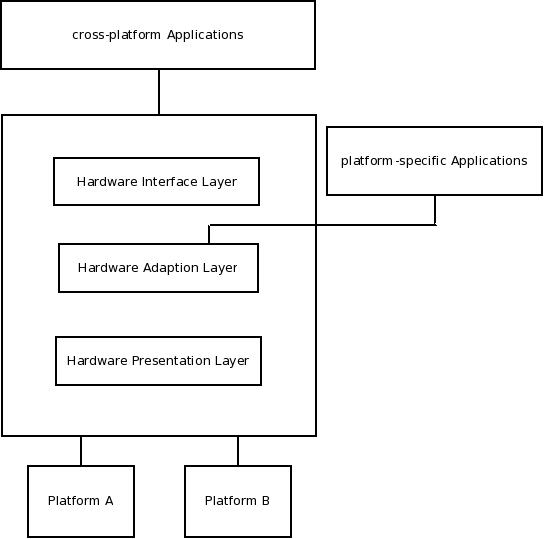
\includegraphics[width=.6\columnwidth]{pics/hardwareabstraction.png}}
  \caption{Hardware Abstraction Architecture}
  \label{fig:haa}
\end{figure}

In contrast to other embedded OS that use only 2 layer abstraction, the third tinyOS layer provides more flexibility. For maximum performance, a \textit{Platform-Specific-Application} can directly hook into the \textit{Hardware Adaption Layer}, circumventing the \textit{Hardware Interface Layer}.


\section{tinyOS internals}

\subsection{Basic - Scheduler}

By default, tinyOS 2.x uses a \textbf{non-preemptive FIFO} scheduler with a maximum of 255 parameterless tasks waiting for execution. A task can only be scheduled once at a time, if periodic execution is needed the task has to re-post itself just before finishing. The scheduler itself consists of an interminable for-loop, that pops ( = executes) one task after the other, in sequence as this tasks got pushed. If no tasks are waiting for execution, the scheduler enters a powersaveing-mode immediatly.

Because the scheduler of tinyOS is implemented as a component it is possible to replace this default FIFO-scheduler with a selfwritten one. See ~\cite{tep106:2003} for details how to implement a selfwritten scheduler.

\subsection{Microcontroller Power Management}

To reduce power consumption, a microcontroller should always run in the lowest power state possible. For example, if you want to run an embedded system that is powered by two AA batteries with a capacitiy of 2.7Ah, for one year, you reach an average of about 1mW of power consumption. Clearly, this can only be achieved by saving energy whenever possible.

As mentioned above, tinyOS enters a low power mode if the task queue is empty. Normally, microcontrollers support a range of low power modes, the ATmega128 - for example - supports up to 6 different power saving modes.
To decide what mode fits best, tinyOS uses the control- and statusregisters to find the proper lowpower-mode.

For example, on a ATmega128-based platform, the cpu-specific powersaving-mode \textit{IDLE} is to be choosen if one or more timer, SPI, UART or I2C are in use. If the ADC-submodule is working, another mode, \textit{ADC Noise Reduction}, is entered. If none of this modules are active and the task queue is empty, the cpu is set to \textit{POWER DOWN}, from which it only can resume by some external interrupts/resets or a SPI address match interrupt.

Because entering powersaving modes always come with wakeup latency, problems can arise if some higher-level hardware modules have timeing constraints if the wakeup latency is too big. To solve this, the powersaving mode, found by examing the control- and statusregisters, can be overridden by a higherlevel module. For example, when going to a sleepmode just befor an alarm of a timer would occur, the wakeup latency could propably cause a miss of this alarm. Therefore, a component can \textit{provide} an interface named \textit{lowestState} that will be called when a powersave mode is requested, and can override the in principle valid powersaveing mode found by looking at the control- and statusregisters.

\subsection{Boot Sequence}

When tinyOS is booting up, it uses 3 interfaces:

\begin{itemize}
 \item Init
 \item Scheduler
 \item Boot
\end{itemize}

\textbf{Init} has one command, called \textit{init()}, that is responsible for initializing hardware components. Initialization must happen sequential, so a component is allowed to use a spin loop when - for example - waiting for an interrupt.
\textbf{Scheduler} is responsible for initializing the task queue.
Finally, \textbf{Boot} signales the completion of the bootup-process to the application.

\subsection{Ressource Arbitration}

One major task of every operating system is the management of available resources, like communication interfaces that are used by different components. tinyOS distinguishes between 3 different kinds of abstractions:

\begin{itemize}
 \item dedicated resources
 \item virtualized resources
 \item shared resources
\end{itemize}

A \textbf{dedicated} resource is a resource which is allocated by one and only one subsystem all the time. Obvious, no sharing policy is needed here. Examples for such resources are counters and interrupts.

\textbf{Virtualized} resources are used by multiple clients through software virtualization. Here, every client interacts like using a dedicated reosource. Because virtualization is done in software, there is no upper bound on the number of clients(apart from memory/efficiency constraints), with all virtualized instances being multiplexed on top of the underlying resource. Clearly, this virtualization 
goes along with cpu-overhead.

For example, this concept is used for timers on ATmega128-based platforms. Every time a new timer is instantiated, tinyOS builds a virtual timer on top of the physical timer 0. 

The \textbf{shared} concept is used for modules that need exclusive access to a resource for some time. An arbiter is responsible for multiplexing between the different clients that want to use the resource. As long as a client \textit{holds} a resource, it has complete access to it. tinyOS arbiters assume that clients are cooperative, that means that a client only acquires a resource when needed, and only holds it as long as needed, releasing it as soon as possible. No concept of preemption is used here, so client B that needs a resource cannot force Client A to release it.  

The arbiter, the centralized place that knows whether a resource is busy or not, is an interface that must be instantiated by every client that wants to use the resource. After that, the client can \textit{request} the resource. The request is queued by the arbiter if the resource is busy. As soon as the resource is available, a special event, \textit{granted}, is signaled to the client, who has now exclusive access to it. It is the client's responsibility to \textit{release} it so soon as possible.
To avoid monopolizing a resource a \textit{request} for a resource is only queued if there is no other request of this client queued yet.


%%
%% = eof =====================================================================
%%
